

%----------------------------------------------------------------------------------------
%	CHAPTER 3: Water
%----------------------------------------------------------------------------------------

\chapter{FLR impacts on water} \label{ch:water}

Water resources are under severe pressure from global drivers such as population growth, climate change, and land use activities, which have transformed most of the planet’s land surface \citep{UNESCO2018}. Deforestation has been linked to extreme floods, extreme droughts and water pollution, since forests can perform eco-hydrological functions, as regulation of water flow and maintenance of water quality \citep{Tambosi2015}. For this reason, FLR has emerged as a feasible solution for water regulation and purification \citep{Banerjee2009}. However, incorporating water services as a criterion in FLR initiatives is still a challenge, due to the complexity of the forest and water relationship: while it is reasonable to expect a positive effect of forest restoration on water quality \citep{Calder2007}, the impacts of forest cover expansion on water quantity are unclear. Here we proposed a new approach to prioritize areas for FLR based on water quality improvement and a methodology to access the impact of large-scale restoration scenarios on Amazon and Atlantic Forest precipitation patterns. 



%-----------------------------------------------------------------------------------------------
\section{\Large Water quality } \label{sec:water-qual}

FLR has direct influence on water quality in freshwater ecosystems. Riparian forests protect soils from erosion and limit sediments and nutrients exportation to water bodies \citep{Neary2009}. When riparian forests are present, nutrients used in agriculture, such as nitrogen and phosphorus, and contaminants, such as pesticides and pathogens, can be adsorbed in the forest soil or taken up by plants and microbes avoiding its transport into the water \citep{Gilliam2011}. Such benefits of riparian forests on water quality makes it a priority area for FLR, as stated in the Brazilian law NVPL. But, does any restoration yield such outcomes? 

In a simulation exercise in the Paraiba do Sul river basin study case, we identified that the spatial allocation of forest restoration in the landscape can either improve or reduce FLR benefits to water quality (see more in Box 3). These results highlighted the importance of spatial planning in FLR initiatives and a demand for new approaches of spatial restoration prioritization, based on water quality improvement. In this sense, we are developing a methodology for spatial prioritization of restoration in the Amazon and Atlantic Forest biomes based on sediment and nutrient retention. 

The ecosystem service of sediment and nutrient retention by native vegetation will be assessed by the InVEST sediment and nutrient delivery models. InVEST is a suite of free, open-source software models used to map and value ecosystem services, developed by The Natural Capital project, which is a partnership between Stanford University, the Chinese Academy of Sciences, the University of Minnesota, The Nature Conservancy, and the World Wildlife Fund. The sediment model aims to map overland sediment generation and delivery to the stream, whereas the nutrient model aims to map nutrient sources from watersheds and their transport to the stream. We will quantify and map the values of sediment and nutrient retention, considering both the actual Land use and cover and a projected scenario where entire biomes are restored. The difference between actual and projected scenarios will result in indexes of the potential sediment and nutrient retention improvement following forest restoration in the Amazon and Atlantic Forest. We are gathering and preparing the dataset to run the InVEST models in partnership with the Natural Capital team. Finally, the prioritization model will be developed using an Integer Linear Programming approach, where the objective function determines how much forest to restore in each planning unit in order to maximize sediment and nutrient retention. 

\newpage

\begin{mybox}{TEEB Project}\label{Box3}\refstepcounter{mybox}

 In this TEEB project we present how spatial planning could guide decision-making to comply with national laws and global restoration agreements in an Atlantic Forest watershed. For that we modeled three alternative scenarios in Paraiba do Sul River Basin-São Paulo: (i) Business As Usual (BAU), with no restoration; (ii) Legal Compliance (LC), where restoration occurs in each rural property; (iii) Sustainable Scenario (SS), where restoration was planned to maximize connectivity and minimize costs, combined with implementation of sustainable productive systems (e.g. AgroForest Systems - AFS) to achieve food security. The restoration scenarios (LC and SS) included the recovery of Permanent Preservation Areas/PPAs (ca. 26.540 ha) and 20\% of medium-large private properties, portion ascribe to the Legal Reserves/LRs (ca. 52.400 ha). We performed field trips, an extensive literature review and applied questionnaires and focus group to gather an overview of the socioeconomic aspects, land use and cover map and perceptions of diverse aspects of the basin, including ecosystem services provision. After an initial assessment, we carry out an ecological and economic valuation of ecosystem services (carbon sequestration, water quality, biodiversity conservation and pollination) using InVest program, which was followed by public policies recommendations to achieve the SS. To evaluate \textbf{water} quality, we modelled soil loss and sediment exportation to water, and as expected, sediment exportation to water was lower in scenarios with forest restoration than in the business-as-usual scenario. However, the different criteria for allocating restoration between scenarios (LC: small fragments of restored forest were scattered across the landscape; SS - larger and continuous fragments were concentrated mostly on the basin’s outskirts, near forest remnants) resulted in different patterns. LC was more efficient in avoiding soil exportation to the Paraiba river than the other scenarios, which meant R\$\ 5 million per year in avoided costs of water treatment and dredging. %(Figure \ref{fig:agua}). 
\end{mybox}


%  \begin{figure}
% \centering
% 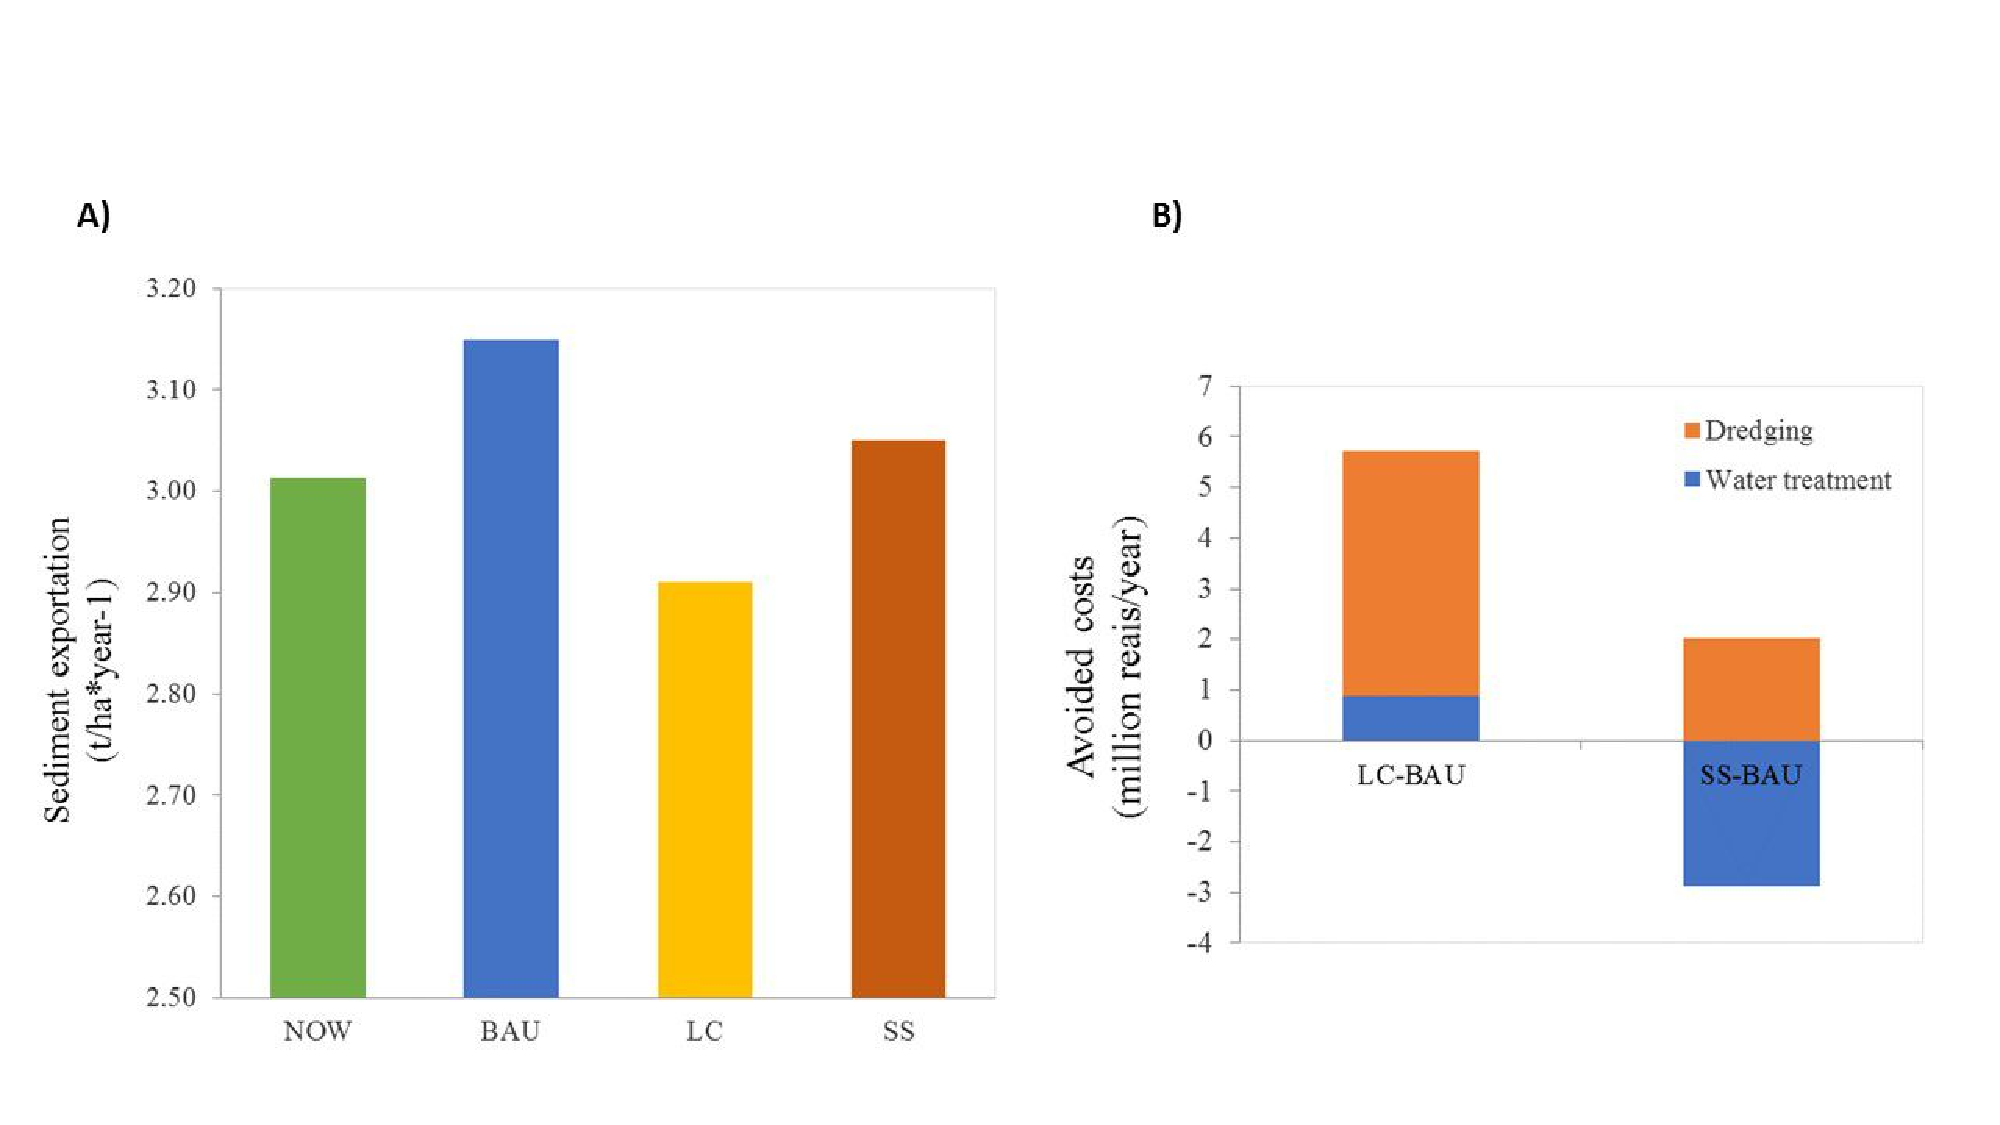
\includegraphics[width=\textwidth]{pictureve/Agua_final.pdf}
% \caption{A) Sediment exportation among scenarios; B) Avoided costs of water treatment and dredging in scenarios with restoration practices \label{fig:agua}}
% \end{figure}


%-----------------------------------------------------------------------------------------------
\section{\Large Water quantity } \label{sec:water-quant}

The prevailing paradigm that vegetation recovery diminishes water availability on terrestrial surfaces requires in-depth examination. Many assessments indicate annual run-off reduction after forest cover expansion on watersheds \citep{Filoso2017}, but a broader picture suggests the opposite is true. The conventional approach for quantifying water production focuses on how precipitation is partitioned over evapotranspiration and run-off at the catchment scale. This approach, however, is not appropriate for assessing the complex impacts of vegetation recovery on water at larger scales \citep{Ellison2012}. It is necessary to understand how different catchments are interconnected and how water, primarily in the form of atmospheric moisture, is transferred across terrestrial surfaces to provide source waters for rainfall at more distant locations \citep{Ellison2018}. \\
\indent Vegetation recovery alters the water balance of a system in multiple ways by affecting several parameters other than annual run-off and the cross- continental transport of atmospheric moisture; e.g. air humidity, soil moisture, groundwater recharge, soil surface and subsurface flows, precipitation patterns and even surface temperatures. These parameters are related to the provision of ecosystem benefits to people at different levels, depending on the environmental constraints and the water uses of local communities. Thus, socioeconomic aspects should be considered as well. In other words, we need to go beyond catchment scale and run-off-based analyses to assess the complete impact of FLR on water-related contributions to people at the catchment and also at the landscape and regional levels. \\
\indent To discuss these questions, we organized and held an international workshop on ‘Restoration and Water’. Experts on forest restoration, ecosystem services, soil science, limnology, modelling, hydrology, climate, and social science were invited. Attendees and lecturers included: Dr. David Ellison (Swedish University of Agricultural Sciences), Dr. Solange Filoso (University of Maryland Center for Environmental Science - UMCES; and National Socio-Environmental Synthesis Center - SESYNC), Dr. Andrian Vogl (Stanford University and natural Capital Project), Dr. Pedro Brancalion, Dr. Paula Meli, and Dr. Miguel Cooper (Luiz de Queiroz College of Agriculture - ESALQ), Dr. Daniel Rodriguez (Alberto Luiz Coimbra Institute for Graduate Studies and Research in Engineering - COPPE/UFRJ), Dr. Sin Chan Chou (National Institute for Space Research - INPE), Dr. Aliny Pires (Brazilian Foundation for Sustainable Development - FBDS), Dr. Vinicius Farjalla (Federal University of Rio de Janeiro - UFRJ), Dr. Alvaro Iribarrem (International Institute for Sustainability -IIS). Organizers: Dr. Bernardo Strassburg (IIS and Pontifical Catholic University of Rio de Janeiro – PUC-Rio), Dr. Agnieszka Latawiek (IIS and Pontifical Catholic University of Rio de Janeiro – PUC-Rio), Dr. Fabio Scarano (FBDS and UFRJ), and MSc. Viviane Dib (IIS and UFRJ).

The workshop outcome was a perspective article (in preparation), in which we aim to frame the links between vegetation recovery and water under a complex and dynamic socio-ecological system, encompassing multiple scales, complex landscape factors, and multiple potential benefits. It will be the first time that information on interactions and trade-offs of these processes will be synthesized considering the entire hydrological space and social elements. This approach will contribute to clarify why estimates in the literature and real-world-case-studies vary widely, and why our ability to predict these interactions are still limited. 

Given that, we expect our results to inform public policies and practitioners on how we can best include water services into restoration planning and implementation, thus reducing risks. Additionally, we discussed methodologies to evaluate the impacts of large-scale restoration scenarios mentioned above (based on biodiversity conservation – section ~\ref{ch:biodiv} and climate mitigation - section ~\ref{ch:carbon}) on the Amazon and Atlantic Forest precipitation patterns. These impacts will be assessed by a coupled atmosphere-surface model developed by the Brazilian National Institute for Space Research – The Eta Model, which allows the assessment of land use and land cover change impacts on local precipitation patterns. 

